\section{The Simple Series archetype}
\begin{frame}
  \frametitle{The simple serie archetype}

  \begin{definition}[Simple serie archetype]
    A series of $n$ neurons $N_1, ..., N_n$, where $N_i$ receives the signal form $N_{i-1}$ and emits its signal to $N_{i+1}$.
  \end{definition}

  \mysep{}

  There exists $2$ main implementations of this archetype:
  \begin{itemize}
    \item the $n$-delayer
    \item the $n$-delayer/filter
  \end{itemize}

\end{frame}

\begin{frame}[fragile]
  \frametitle{The $n$-delayer}

  Given a signal $\mathcal{S}$, $\mathcal{S}$ is transmitted with a delay of $n$ time units.

  \mysep{}

  Simple implementation:

  \begin{figure}
    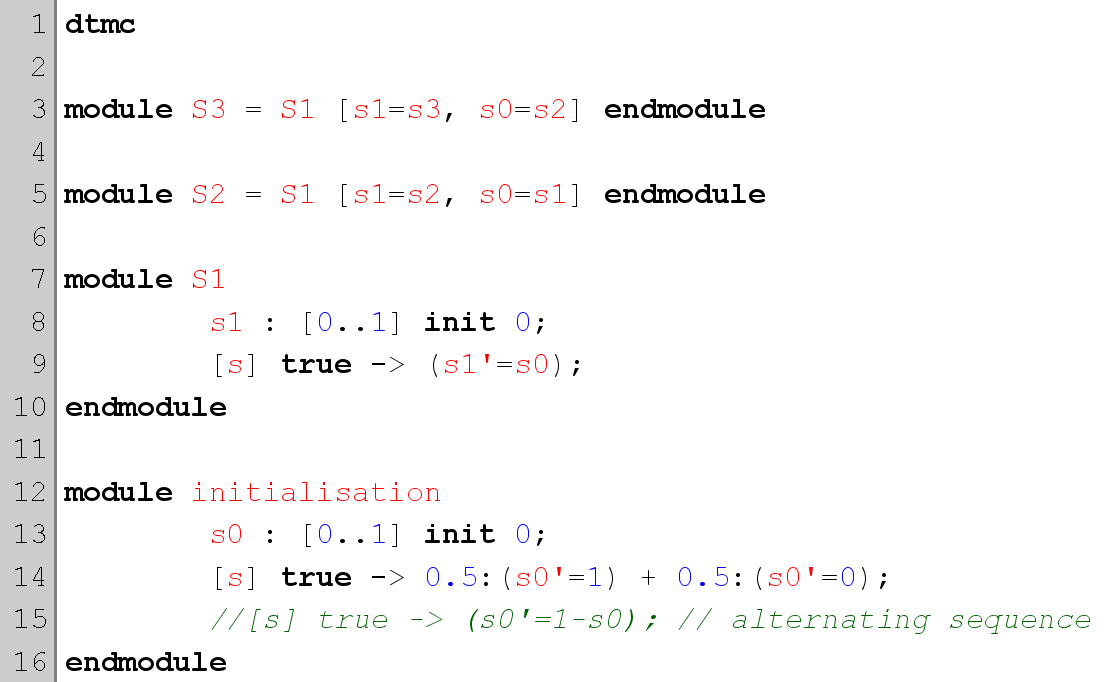
\includegraphics[width=0.7\textwidth]{pic/simple_serie1_code.png}
  \end{figure}

\end{frame}

\begin{frame}
  \frametitle{A plot of a $n$-delayer}

  \begin{figure}
    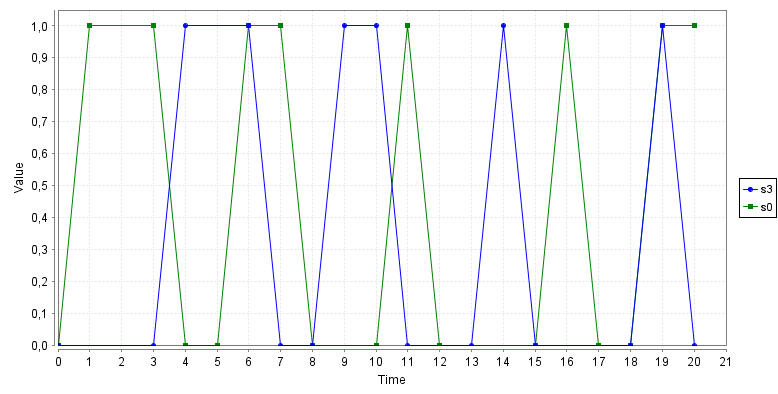
\includegraphics[width=0.8\textwidth]{pic/simple_serie1_plot.png}
  \end{figure}

  \mysep{}

  An interesting property:
  \begin{itemize}
    \item $P \stackrel{?}{=} [G (s_0 = 1 \Leftrightarrow (X^3 s_3=1))] $ \uncover<2->{Answer: $1.0$}
  \end{itemize}

\end{frame}

\begin{frame}
  \frametitle{The $n$-delayer/filter}

  Let's introduce the leak factor and the potential membrane: an example of code corrector.

  \begin{figure}
    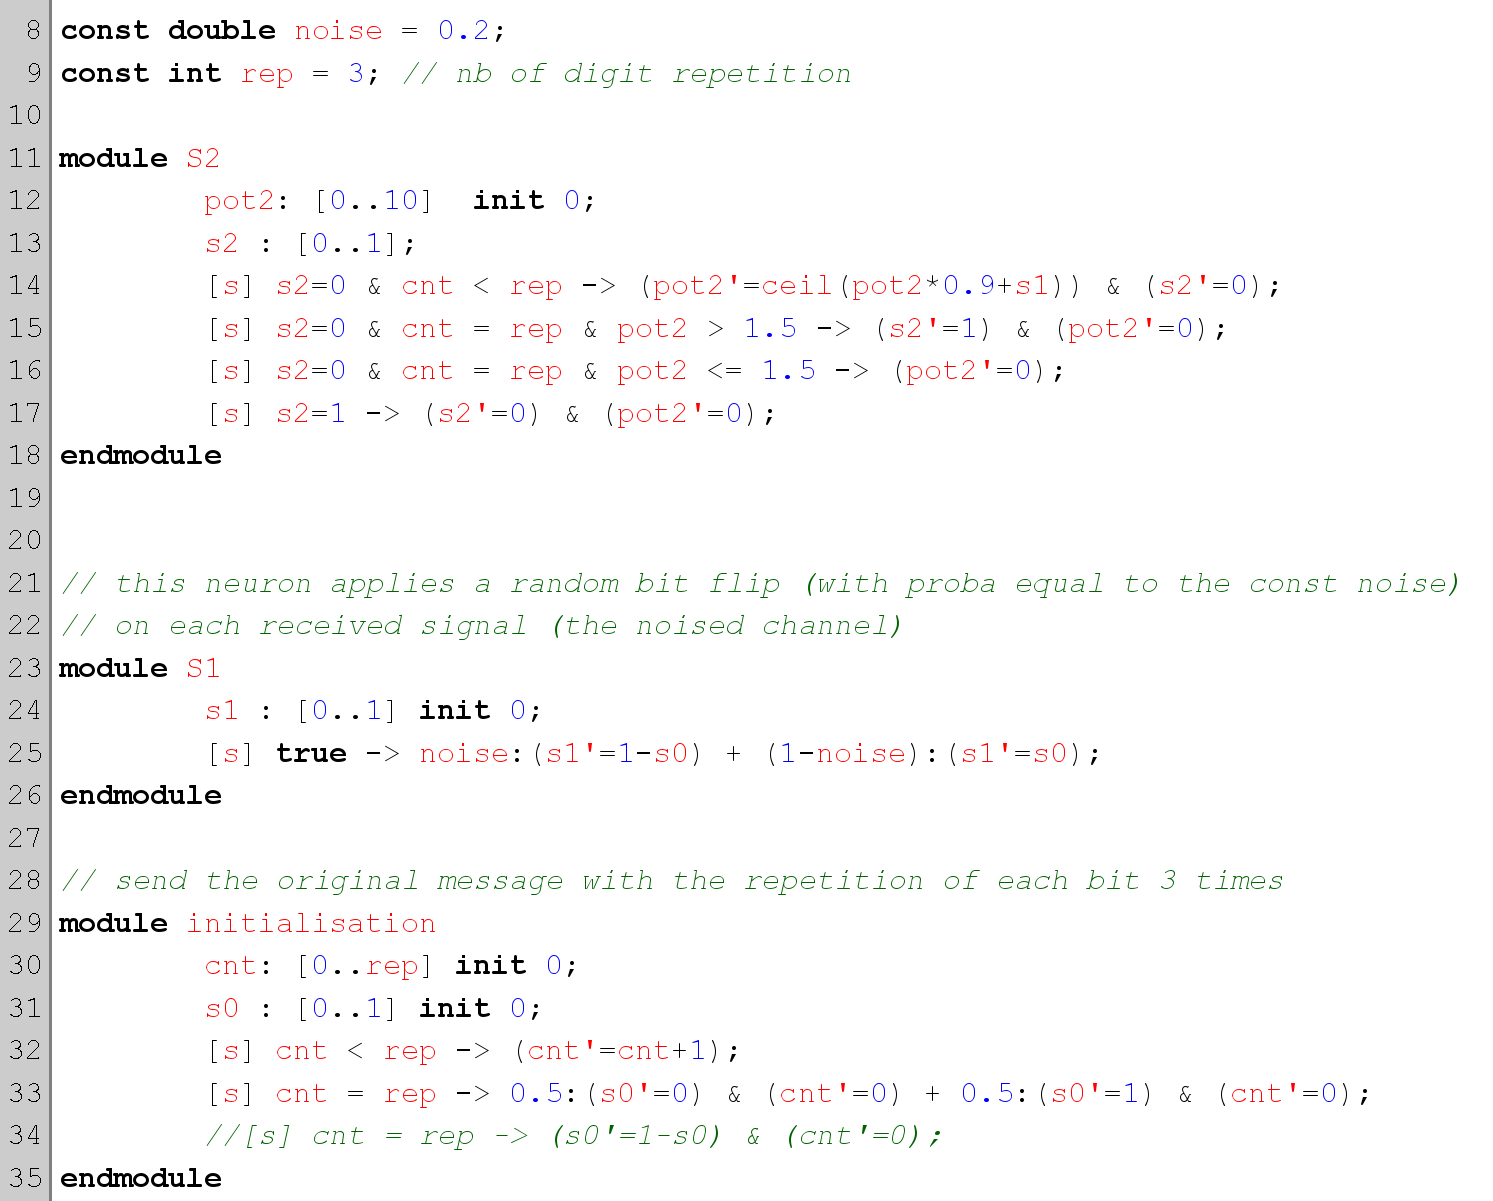
\includegraphics[width=0.62\textwidth]{pic/simple_serie_corr_code.png}
  \end{figure}

\end{frame}

\begin{frame}
  \frametitle{A plot of a $n$-delayer/filter}

  \begin{figure}
    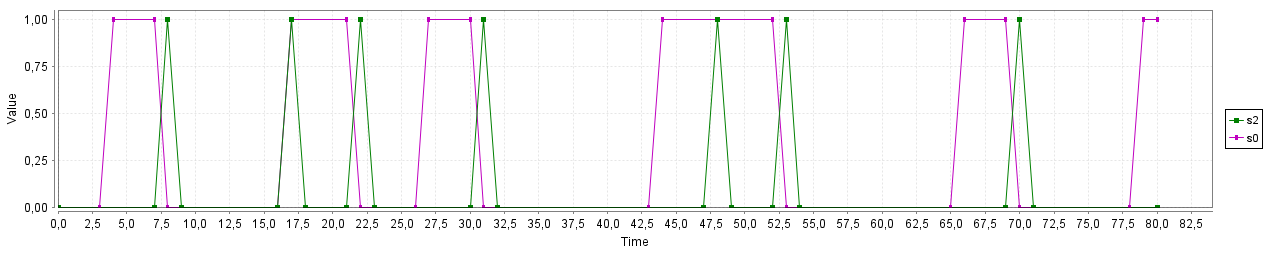
\includegraphics[width=0.9\textwidth]{pic/simple_serie_corr_plot.png}
  \end{figure}

  \begin{figure}
    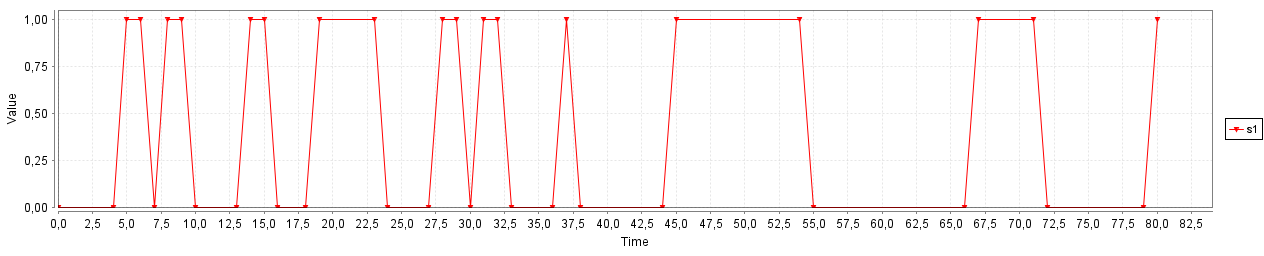
\includegraphics[width=0.9\textwidth]{pic/simple_serie_corr_plot_s1.png}
  \end{figure}

\end{frame}

\begin{frame}
  \frametitle{Test certainty of model by noise}
  \begin{align*}
    P \stackrel{?}{=} &
    \begin{cases}
      (X^4 ((s_0=1) \Leftrightarrow X^5 (s_2=1))) & \text{if } noise > 0.5 \\
      (X^4 ((s_0=1) \Leftrightarrow X^4 (s_2=1))) & \text{otherwise}
    \end{cases}
  \end{align*}



  \begin{columns}
    \begin{column}{0.45\textwidth}
      \begin{table}[]
        \begin{tabular}{cc}
          noise  & proba  \\ \hline
          $0.00$ & $1.00$ \\
          $0.10$ & $0.90$ \\
          $0.50$ & $0.50$ \\
          $0.90$ & $0.18$ \\
          $1.00$ & $0.00$
        \end{tabular}
      \end{table}
    \end{column}
    \begin{column}{0.45\textwidth}  %%<--- here
      \begin{remark}
        If the $noise$ is bigger than $0.5$, we have to look at the fifth time-unit: one time-unit is consumed by the $reset$ action.
      \end{remark}
    \end{column}
  \end{columns}

\end{frame}

\begin{frame}
  \frametitle{A complete example}

  \begin{figure}
    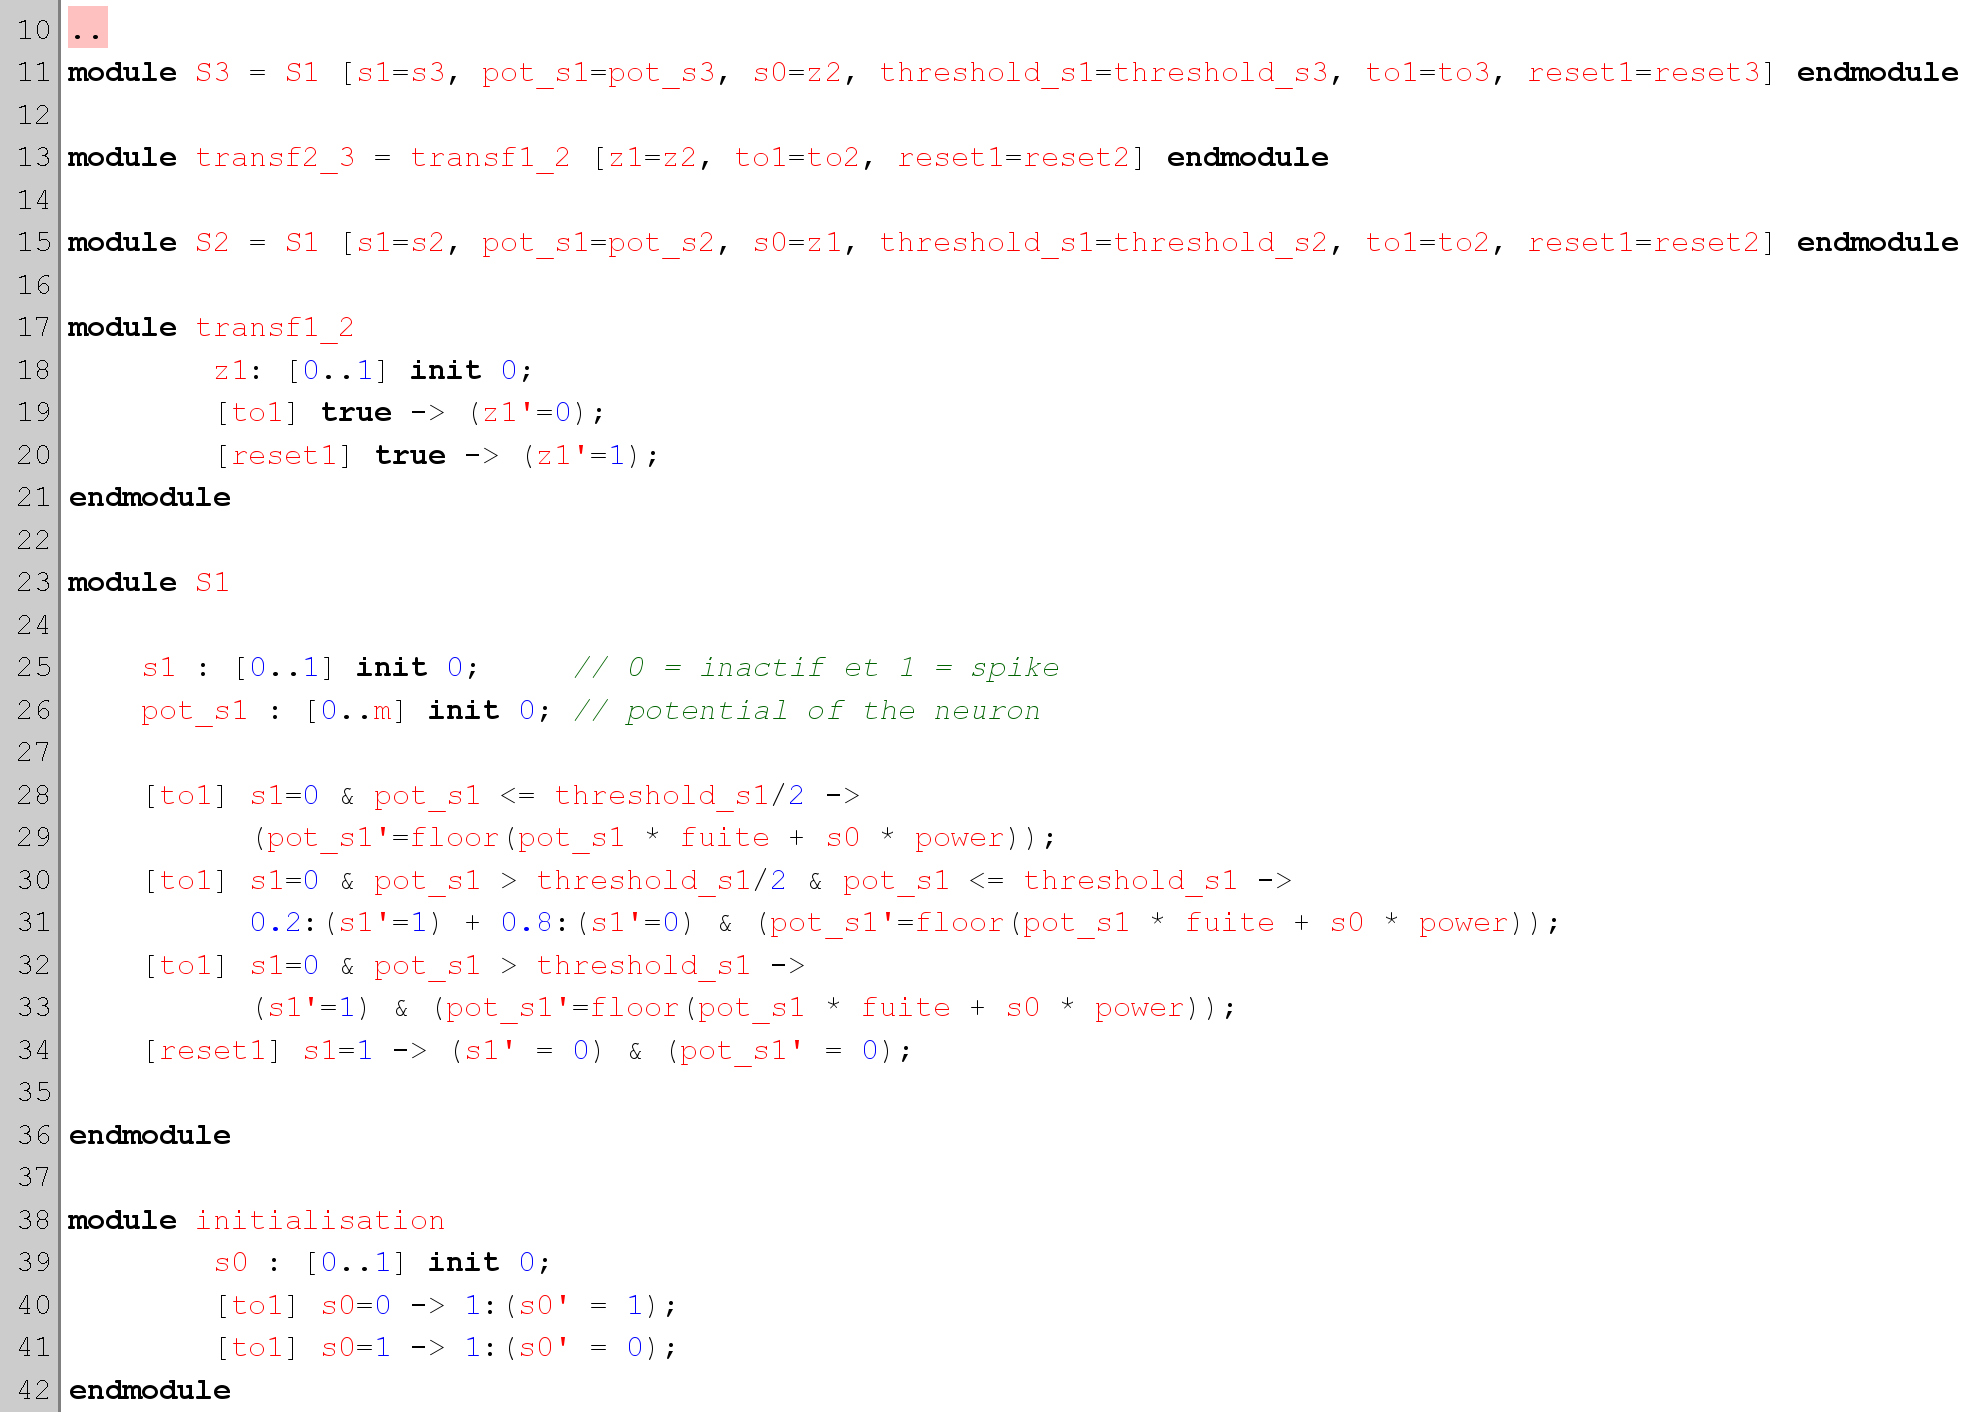
\includegraphics[width=0.8\textwidth]{pic/simple_serie_complex.png}
  \end{figure}

\end{frame}

\begin{frame}
  \frametitle{A corresponding plot}

  \begin{figure}
    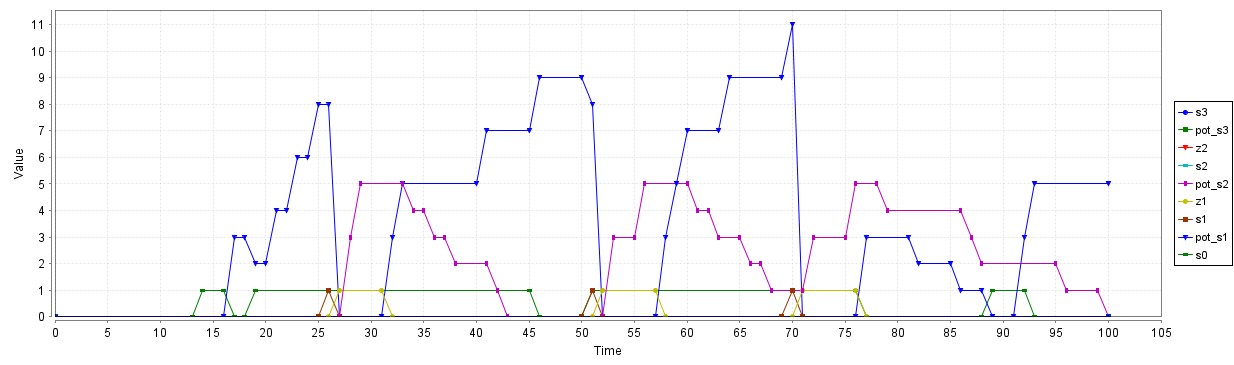
\includegraphics[width=\textwidth]{pic/simple_serie_complex_plot.png}

    \includegraphics<2>[width=\textwidth]{pic/simple_serie_complex_explorat.png}
  \end{figure}

\end{frame}